\documentclass[spanish]{beamer}

%%% CODIFICACIÓN

\usepackage[utf8]{inputenc}
\usepackage[spanish]{babel}
\usepackage{graphics,tikz}
\graphicspath{{./fig/}}
\usepackage{caption}
\usepackage{subcaption}
%%% FUENTES

\usepackage[T1]{fontenc}
\usepackage[familydefault,regular]{}
\usepackage{newtxsf} % Fuente de matemáticas

\setbeamertemplate{navigation symbols}{}

%%% COLORES

\definecolor{background}{RGB}{255,255,255}
\definecolor{text}{RGB}{78,78,78}
\definecolor{accent}{RGB}{6, 105, 125}

\setbeamerfont{framesubtitle}{size=\normalfont\tiny}
\setbeamercolor{framesubtitle}{fg=white}

%%% Matemáticas
\usepackage{amsmath}
\usepackage{amssymb}
\usepackage{amsbsy}
\usepackage{tipa}
\newcommand{\norm}[1]{\left\lVert#1\right\rVert}
\newcommand{\yy}{\textbf{y}}
\usepackage{blkarray}

%%% Código
\usepackage{listings}

%%% Tablas
\usepackage{tabularx}
\usepackage{float}
\usepackage{adjustbox}
\usepackage{booktabs}
\usepackage{array}
\newcolumntype{L}[1]{>{\raggedright\let\newline\\\arraybackslash\hspace{0pt}}m{#1}}
\newcolumntype{C}[1]{>{\centering\let\newline\\\arraybackslash\hspace{0pt}}m{#1}}
\newcolumntype{R}[1]{>{\raggedleft\let\newline\\\arraybackslash\hspace{0pt}}m{#1}}

%%% AJUSTES DE BEAMER

% ¿Negrita en el título de diapositiva o no?
%\setbeamertemplate{frametitle}{\color{accent}\vspace*{1cm}\bfseries\insertframetitle\par\vskip-6pt}

\setbeamertemplate{frametitle}{\color{accent}\vspace*{1cm}\insertframetitle\par\vskip-6pt}

\setbeamertemplate{itemize items}[circle] % Viñetas de itemize

%%% CONFIGURACIÓN DE COLORES DE BEAMER

\setbeamercolor{background canvas}{bg=background}
\setbeamercolor{normal text}{fg=text}
\setbeamercolor{alerted text}{fg=accent}
\setbeamercolor{block title}{fg=accent}
\setbeamercolor{alerted text}{fg=accent}
\setbeamercolor{itemize item}{fg=accent}
\setbeamercolor{enumerate item}{fg=accent}
\setbeamercolor*{title}{fg=accent}
\setbeamercolor{caption name}{fg=accent}
\setbeamercolor{qed symbol}{fg=accent}
\setbeamercolor{itemize subitem}{fg=accent}
\setbeamercolor{bibliography entry author}{fg=text}
\setbeamertemplate{itemize subitem}[triangle]
\usebeamercolor[fg]{normal text}

%%% SECTIONS
\setbeamercolor{mycolor}{fg=white,bg=accent}

\AtBeginSection[]{
  \begin{frame}
  \vfill
  \centering
  \begin{beamercolorbox}[sep=8pt,center,shadow=true,rounded=true]{mycolor}%
    \usebeamerfont{title}\insertsectionhead\par%
  \end{beamercolorbox}
  \vfill
  \end{frame}
}



%%% INFORMACIÓN DEL DOCUMENTO

\title{\textit{Clustering}}
\subtitle{Estadística Multivariante}
\author{Sofía Almeida Bruno\\ Daniel Bolaños Martínez\\ José María Borrás Serrano\\ Fernando de la Hoz Moreno\\ Pedro Manuel Flores Crespo\\ María Victoria Granados Pozo}


\begin{document}

\maketitle
	
\begin{frame}{\textit{Clustering}}
  \begin{itemize}
  \item Objetivo: agrupar objetos similares.
  \item Dadas \textbf{$x_1$}$,\cdots, $\textbf{$x_n$} medidas de $p$ variables en $n$ objetos considerados \textit{heterogéneos}. El objetivo del análisis clúster es agrupar estos objetos en $k$ clases \textit{homogéneas}, donde $k$ es también desconocido.
  \end{itemize}
\end{frame}

\begin{frame}{\textit{Clustering}}
\begin{figure}[H]
	\centering
	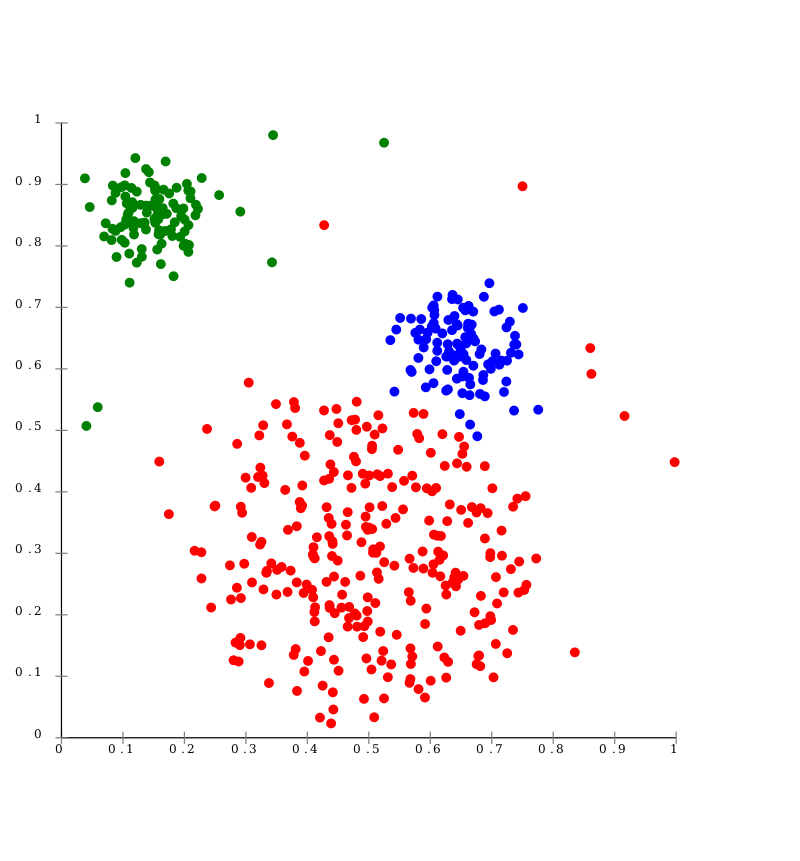
\includegraphics[scale=0.2]{ejemplo}
	\caption{Ejemplo de \textit{clustering}. \cite{chire_deutsch:_2011}}
	\label{fig:ejemplo1}
\end{figure}
\end{frame}

\begin{frame}{Ejemplos de \textit{Clustering}}
  \begin{itemize}
  \item Biología: determinación de especies.
  \item \textit{Marketing}: descubrimiento de grupos de clientes.
    \begin{figure}[H]
	\centering
	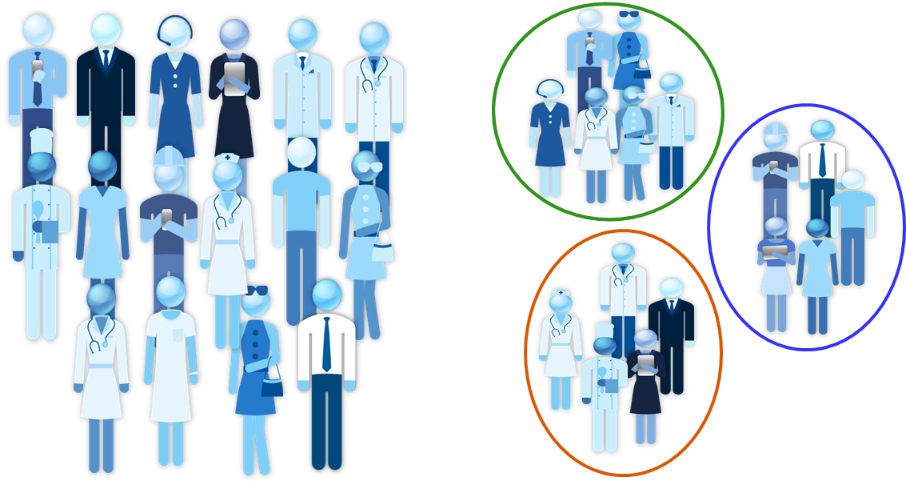
\includegraphics[scale=0.5]{ej_marketing}
	\caption{Ejemplo de \textit{clustering}. \cite{noauthor_understanding_nodate}}
\end{figure}
  \item Psicología: encontrar tipos de personalidad.
  \item Arqueología: datar objetos encontrados.
  \item Planificación urbana: identificar grupos de viviendas.
  \end{itemize}
\end{frame}

\begin{frame}{\textit{Clustering}}
  Para realizar un análisis clúster hay que:
  \begin{itemize}
  \item Elegir una medida de similitud.
  \item Elegir un algoritmo para construir los grupos.
    \begin{itemize}
    \item Particionamiento.
    \item Jerárquicos.
    \end{itemize}
  \end{itemize}
\end{frame}

\section{Medidas de similitud}

\begin{frame}{\textit{Medidas de similitud}}

Realizar un agrupamiento simple a partir de un conjunto complejo de datos requiere una medida de ``similitud''.\break

Para elegir esta medida es necesario tomar consideraciones iniciales como:

\begin{itemize}
\item Naturaleza de las variables (discreta, continua, binaria).
\item Escalas de las medidas (nominal, ordinal, intervalo).
\item Conocimiento sobre el problema.
\end{itemize}\

Los valores de las variables consideradas deberán ser normalizados.
\end{frame}

\begin{frame}{\textit{Distancias de similitud para pares de ítems}}

La distancia estadística entre dos observaciones $p$-dimensionales $x^T = [x_1,\dots,x_p]$ e $y^T=[y_1,\dots,y_p]$ es:

$$d(x,y)=\sqrt{(x-y)^TA(x-y)} $$

Donde $A=S^{-1}$ y $S$ contiene las varianzas y covarianzas de la muestra.
$S$ no es conocida antes de aplicar clustering, por lo que se suele usar la distancia euclídea:

$$d(x,y) = \sqrt{(x_1-y_1)^2+\dots+(x_p-y_p)^2}=\sqrt{(x-y)^T(x-y)}.$$
\end{frame}

\begin{frame}{\textit{Otras medidas y coeficientes de similitud}}

\begin{itemize}
\item Métrica de Minkowski:
$$ d(x,y)=\left  [\sum_{i=1}^{p}{|x_i-y_i|^m} \right ]^{1/m}$$
\item Métrica de Canberra (variables no negativas):
$$d(x,y)=\sum_{i=1}^{p}{\frac{|x_i-y_i|}{(x_i+y_i)}}$$
\item Coeficiente de Czekanowski (variables no negativas):
$$d(x,y)=1-\frac{2\sum_{i=1}^{p}{min(x_i,y_i)}}{\sum_{i=1}^{p}{(x_i+y_i}}$$
\end{itemize}
\end{frame}

\begin{frame}{\textit{Binarización de variables}}

Si los ítems no pueden ser representados por medidas $p$-dimensionales significativas, las parejas de ítems se suelen comparar según la presencia o ausencia de ciertas características.\break

Matemáticamente se consigue introduciendo una variable binaria, que toma el valor 1 si la característica está presente y el valor 0 si no. 

\begin{table}[h]
\centering
  \begin{tabular}{lrrrrr}
    \toprule
  Variables    & 1    & 2    & 3   & 4   & 5   \\
  \midrule
Ítem $i$ & 1    & 0    & 0   & 1   & 1   \\
Ítem $k$ & 1    & 1    & 0   & 1   & 0\\
\bottomrule
\end{tabular}
\end{table}
\end{frame}

\begin{frame}{}

Sea $x_{ij}$ la puntuación de la $j$-ésima variable binaria en el $i$-ésimo ítem y $x_{kj}$ la de la $j$-ésima en el $k$-ésimo ítem, con $j=1,\dots,p$. Entonces:

$$(x_{ij}-x_{kj})^2 = \left \{ \begin{matrix} 0 & \mbox{si } x_{ij}=x_{kj}
\\ 1 & \mbox{si }x_{ij}\neq x_{kj}\end{matrix}\right.   $$

y $\sum_{j=1}^p{(x_{ij}-x_{kj})^2}$ proporciona una forma de contar el número de disparidades. Una distancia grande corresponde a muchas disparidades, es decir, ítems desemejantes.\break 

En el Ejemplo anterior:

$$\sum_{j=1}^5{(x_{ij}-x_{kj})^2}=(1-1)^2+(0-1)^2+(0-0)^2+(1-1)^2+(1-0)^2=2.$$
\end{frame}

\begin{frame}{\textit{Problemas de la distancia usada}}
La distancia usada valora por igual las parejas 1-1 y 0-0. En algunos casos no es cierto.\break 

Existen diversos esquemas para definir los coeficientes de similitud. Organizando las frecuencias de las parejas que coinciden y las que no para los ítems $i$ y $k$ en forma de tabla de contingencia:

\begin{table}[H]
  \centering
\resizebox{7cm}{!} {
  \begin{tabular}{llrrrrr}
\multicolumn{2}{l}{\multirow{}{}{}} & \multicolumn{3}{c}{Ítem $k$} & \multicolumn{2}{c}{} \\\cmidrule{3-5}
\multicolumn{2}{l}{}                  & 1        &       & 0       & \multicolumn{2}{c}{{Total}}                        \\
\midrule
{Ítem $i$}       & 1      & $a$        &       & $b$       & \multicolumn{2}{c}{$a+b$}                     \\
                              & 0      & $c$        &       & $d$       & \multicolumn{2}{c}{$c+d$}                     \\ \midrule
\multicolumn{2}{l}{Total}            & $a+c$      &       & $b+d$     & \multicolumn{2}{c}{$p=a+b+c+d$}\\
\bottomrule
\end{tabular}
}
\end{table}

\end{frame}

\begin{frame}{}

\begin{table}[H]
  \centering
  \caption{Coeficientes de similitud para ítems \textit{clustering}.}
\resizebox{10cm}{!} {
\begin{tabular}{ll}
\toprule               
\multicolumn{1}{l}{Coeficiente} & \multicolumn{1}{l}{Fundamento}\\
\midrule
1 $\quad\frac{a+d}{p}$                            & Las parejas 1-1 y 0-0 ponderan lo mismo.\\ \\
2 $\quad\frac{2(a+d)}{2(a+d)+b+c}$                            & Las parejas 1-1 y 0-0 ponderan el doble.                                                                                                        \\\\
3 $\quad\frac{a+d}{a+d+2(b+c)}$                             & Las parejas que no coinciden ponderan el doble.                                                                                                 \\\\
4  $\quad\frac{a}{p}$                             & No hay parejas 0-0 en el numerador.                                                                                                    \\         \\
\bottomrule
\end{tabular}
}
\end{table}

\end{frame}

\begin{frame}{}
\begin{table}[H]
  \centering
  \caption{Coeficientes de similitud para ítems \textit{clustering}.}
\resizebox{10cm}{!} {
\begin{tabular}{ll}
\toprule               
\multicolumn{1}{l}{Coeficiente} & \multicolumn{1}{l}{Fundamento}\\
\midrule
5 $\quad\frac{a}{a+b+c}$                             & \begin{tabular}[c]{@{}l@{}}No hay parejas 0-0 en el numerador ni el denominador\\ (Las parejas 0-0 son irrelevantes).\end{tabular}              \\\\
6 $\quad\frac{2a}{2a+b+c}$                             & \begin{tabular}[c]{@{}l@{}}No hay parejas 0-0 en el numerador ni el denominador.\\ Las parejas 1-1 ponderan el doble.\end{tabular}              \\\\
7 $\quad\frac{a}{a+2(b+c)}$                             & \begin{tabular}[c]{@{}l@{}}No hay parejas 0-0 en el numerador ni el denominador.\\ Las parejas que no coinciden ponderan el doble.\end{tabular} \\\\
8 $\quad\frac{a}{b+c}$                             & \begin{tabular}[c]{@{}l@{}}Proporción de parejas que coinciden (excluyendo las 0-0) en\\  relación a las parejas que no coinciden.\end{tabular} \\\\
\bottomrule
\end{tabular}
}
\end{table}
\end{frame}

\begin{frame}{\textit{Ejemplo de cálculo de coeficientes de similitud}}
Veamos un ejemplo de cálculo de coeficientes de similitud.\break

Definiremos 5 individuos con diferentes características y 6 variables binarias $X_1,X_2,X_3,X_4,X_5,X_6$.
\begin{table}[h]
  \centering
  \label{tab:ej-similitud}
\resizebox{11cm}{!} {
  \begin{tabular}{lrrrrrr}
    \toprule
            & Altura (in) & Peso (lb) & Color de ojos & Color de pelo & Mano predominante & Género \\ \midrule
Individuo 1 & 68                       & 140                    & Verde                             & Rubio                             & Derecha                               & Femenino\\
Individuo 2 & 73 & 185 & Marrón & Moreno & Derecha & Masculino                  \\
Individuo 3 & 67 & 165 & Azul & Rubio & Derecha & Masculino                  \\
Individuo 4 & 64 & 120 & Marrón & Moreno                            & Derecha & Femenino \\
Individuo 5 & 76 & 210 & Marrón & Moreno & Izquierda & Masculino\\                 
\bottomrule
\end{tabular}
}
\end{table}
\end{frame}

\begin{frame}{}
$$X_1 = \left \{ \begin{matrix} 1 & \mbox{si Altura}  \geq 72 
\\ 0 & \mbox{si Altura}  < 72 \end{matrix}\right.$$
$$X_2 = \left \{ \begin{matrix} 1 & \mbox{si Peso}  \geq 150 
\\ 0 & \mbox{si Peso}  < 150 \end{matrix}\right.   $$
$$X_3 = \left \{ \begin{matrix} 1 & \mbox{si Ojos marrones} 
\\ 0 & \mbox{si otro color de ojos}\end{matrix}\right.   $$
$$X_4 = \left \{ \begin{matrix} 1 & \mbox{si Pelo rubio} 
\\ 0 & \mbox{si otro color de pelo } \end{matrix}\right.   $$

$$X_5 = \left \{ \begin{matrix} 1 & \mbox{si Diestro} 
\\ 0 & \mbox{si Zurdo } \end{matrix}\right.   $$

$$X_6 = \left \{ \begin{matrix} 1 & \mbox{si Masculino} 
\\ 0 & \mbox{si Femenino}  \end{matrix}\right.   .$$
\end{frame}

\begin{frame}{}
Las puntuaciones de los individuos 1 y 2 en las $p=6$ variables binarias se muestran a continuación:\break

\begin{table}[h]
  \centering
\resizebox{8cm}{!} {
  \begin{tabular}{lrrrrrr}
    \toprule
            & \multicolumn{1}{l}{$X_1$} & \multicolumn{1}{l}{$X_2$} & \multicolumn{1}{l}{$X_3$} & \multicolumn{1}{l}{$X_4$} & \multicolumn{1}{l}{$X_5$} & \multicolumn{1}{l}{$X_6$} \\ \midrule
Individuo 1 & 0                        & 0                        & 0                        & 1                        & 1                        & 1                        \\
Individuo 2 & 1                        & 1                        & 1                        & 0                        & 1                        & 0\\
\bottomrule
\end{tabular}
}
\end{table}
\end{frame}

\begin{frame}
El número de parejas que coinciden y las que no se indican a continuación en la tablas de contingencias:
\begin{table}[h]
  \centering
  \label{tab:contingencias-ej}
\resizebox{6.5cm}{!} {
  \begin{tabular}{lrrrrr}
\multicolumn{2}{l}{\multirow{}{}{}} & \multicolumn{2}{c}{Individuo 2} & \\\cmidrule{3-4}
\multicolumn{2}{l}{}                  & 1        &   0       & \multicolumn{2}{c}{Total}                        \\ \midrule
Individuo 1      & 1      & 1        &  2       & \multicolumn{2}{c}{3}                     \\
                              & 0      & 3        &    0       & \multicolumn{2}{c}{3}                     \\ \midrule
\multicolumn{2}{l}{Total}            & 4     & 2     & \multicolumn{2}{c}{6}\\
\bottomrule
\end{tabular}
}
\end{table}\

Empleando el primer coeficiente de similitud de la tabla, calculamos:

$$\frac{a+d}{p}=\frac{1+0}{6}=\frac{1}{6}. $$
\end{frame}

\begin{frame}{}
Calcularemos los demás números de similitud para cada pareja de individuos. Mostramos los resultados en la matriz simétrica 5 x 5.

\begin{table}[H]
\centering
\resizebox{9cm}{!} {
\begin{tabular}{lllllll}
\multicolumn{2}{l}{\multirow{}{}{}}               & \multicolumn{5}{c}{Individuo}                  \\
\multicolumn{2}{l}{}                                & 1   & 2   & 3   & 4   & 5                      \\ \cline{3-3} \cline{7-7} 
\multirow{}{}{Individuo} & \multicolumn{1}{l|}{1} & 1   &     &     &     & \multicolumn{1}{l|}{}  \\
                           & \multicolumn{1}{l|}{2} & 1/6 & 1   &     &     & \multicolumn{1}{l|}{}  \\
                           & \multicolumn{1}{l|}{3} & 4/6 & 3/6 & 1   &     & \multicolumn{1}{l|}{}  \\
                           & \multicolumn{1}{l|}{4} & 4/6 & 3/6 & 2/6 & 1   & \multicolumn{1}{l|}{}  \\
                           & \multicolumn{1}{l|}{5} & 0   & 5/6 & 2/6 & 2/6 & \multicolumn{1}{l|}{1} \\ \cline{3-3} \cline{7-7} 
\end{tabular}
}
\end{table}\

Los individuos 2 y 5 son los más similares mientras que los individuos 1 y 5 son los menos similiares.
\end{frame}

\begin{frame}{Construcción de similitudes a partir de distancias}

Fijamos:

$$ s_{ik} = \frac{1}{1+d_{ik}},$$ 

donde $0<s_{ik}\leq 1$ es la similitud entre los ítems $i$ y $k$, entonces $d_{ik}$ es la distancia correspondiente.\break

No siempre podemos construir distancias ``verdaderas'', a partir de similitudes. Sólo si la matriz de similitudes es definida no negativa y la máxima similitud cumple $s_{ii}=1$.\break

Entonces $ d_{ik}=\sqrt{2(1-s_{ik})}$, cumple las propiedades de una distancia.
\end{frame}

\begin{frame}{\textit{Medidas de similitud para pares de variables}}
Para algunas aplicaciones, son las variables, en lugar de los ítems, las que deben ser agrupadas. Las medidas de similitud para variables suelen tomar la forma de coeficientes de correlaciones muestrales.\break

Cuando las variables son binarias, los datos se pueden organizar en una tabla de contingencia que tiene la siguiente forma:

\begin{table}[h]
  \centering
\resizebox{7.5cm}{!} {
\begin{tabular}{llrrrr}
\multicolumn{2}{l}{\multirow{}{}{}} & \multicolumn{2}{c}{Variable $k$} & \multicolumn{2}{c}{\multirow{}{}{Total}} \\\cmidrule{3-4}
\multicolumn{2}{l}{}                  & 1             & 0       & \multicolumn{2}{c}{}                        \\ \hline
\multirow{}{}{Variable $i$}       & 1      & $a$          & $b$       & \multicolumn{2}{c}{$a+b$}                     \\
                              & 0      & c            & $d$       & \multicolumn{2}{c}{$c+d$}                     \\ \hline
\multicolumn{2}{l}{Total}            & $a+c$          & $b+d$     & \multicolumn{2}{c}{$n=a+b+c+d$}\\
\bottomrule            
\end{tabular}
}
\end{table}
\end{frame}

\begin{frame}{}
La fórmula del coeficiente de correlación producto-momento aplicada a las variables binarias de la tabla de contingencia nos da:

$$r = \frac{ad-bc}{[(a+b)(c+d)(a+c)(b+d)]^{1/2}}.$$\

Podemos tomar $r$ como la medida de similitud entre las dos variables.\break

Se cumple la relación ($r^2=\chi^2/n$) para evaluar la independencia de dos variables categóricas. Para un $n$ fijo, una similitud (o correlación) grande es consistente con la presencia de dependencia.
\end{frame}

\begin{frame}{Ejemplo idiomas}
Medimos las similitudes de 11 lenguajes en base a los primeros 10 números naturales en cada idioma.

\begin{table}[h]
\centering
\resizebox{11.3cm}{!} {
  \begin{tabular}{lllllllllll}
    \toprule
\begin{tabular}[c]{@{}l@{}}Inglés\\ (E)\end{tabular} & \begin{tabular}[c]{@{}l@{}}Noruego\\ (N)\end{tabular} & \begin{tabular}[c]{@{}l@{}}Danés\\ (Da)\end{tabular} & \begin{tabular}[c]{@{}l@{}}Holandés\\ (Du)\end{tabular} & \begin{tabular}[c]{@{}l@{}}Alemán\\ (G)\end{tabular} & \begin{tabular}[c]{@{}l@{}}Francés\\ (Fr)\end{tabular} & \begin{tabular}[c]{@{}l@{}}Español\\ (Sp)\end{tabular} & \begin{tabular}[c]{@{}l@{}}Italiano\\ (I)\end{tabular} & \begin{tabular}[c]{@{}l@{}}Polaco\\ (P)\end{tabular} & \begin{tabular}[c]{@{}l@{}}Húngaro\\ (H)\end{tabular} & \begin{tabular}[c]{@{}l@{}}Finés\\ (Fi)\end{tabular} \\ \midrule
one                                                  & en                                                    & en                                                   & een                                                     & eins                                                 & un                                                     & uno                                                    & uno                                                    & jeden                                                & egy                                                   & yksi                                                 \\
two                                                  & to                                                    & to                                                   & twee                                                    & zwei                                                 & deux                                                   & dos                                                    & due                                                    & dwa                                                  & ketto                                                 & kaksi                                                \\
three                                                & tre                                                   & tre                                                  & drie                                                    & drei                                                 & trois                                                  & tres                                                   & tre                                                    & trzy                                                 & harom                                                 & kolme                                                \\
four                                                 & fire                                                  & fire                                                 & vier                                                    & vier                                                 & quatre                                                 & cuatro                                                 & quattro                                                & cztery                                               & negy                                                  & nelja                                                \\
five                                                 & fem                                                   & fem                                                  & vijf                                                    & funf                                                 & cinq                                                   & cinco                                                  & cinque                                                 & piec                                                 & ot                                                    & viisi                                                \\
six                                                  & seks                                                  & seks                                                 & zes                                                     & sechs                                                & six                                                    & seis                                                   & sei                                                    & szesc                                                & hat                                                   & kuusi                                                \\
seven                                                & sju                                                   & syv                                                  & zeven                                                   & sieben                                               & sept                                                   & siete                                                  & sette                                                  & siedem                                               & het                                                   & seitseman                                            \\
eight                                                & atte                                                  & otte                                                 & acht                                                    & acht                                                 & huit                                                   & ocho                                                   & otto                                                   & osiem                                                & nyolc                                                 & kahdeksan                                            \\
nine                                                 & ni                                                    & ni                                                   & negen                                                   & neun                                                 & neuf                                                   & nueve                                                  & nove                                                   & dziewiec                                             & kilenc                                                & yhdeksan                                             \\
ten                                                  & ti                                                    & ti                                                   & tien                                                    & zehn                                                 & dix                                                    & diez                                                   & dieci                                                  & dziesiec                                             & tiz                                                   & kymmenen                                             \\ \bottomrule
\end{tabular}
}
\end{table}
\end{frame}

\begin{frame}{}
Vemos que inglés, noruego, danés, holandés y alemán parecen formar un grupo. El francés, español, italiano y polaco forman otro, mientras que el húngaro y el finés no forman parte de ninguno.
\begin{table}[h]
\centering
\makebox[\textwidth][c]{
\begin{tabular}{lrrrrrrrrrrr}
\\
\toprule
       & E      & N      & Da     & Du     & G     & Fr    & Sp    & I     & P     & H     & Fi    \\ \midrule
E      & 10     &        &        &        &       &       &       &       &       &       &       \\
N      & 8      & 10     &        &        &       &       &       &       &       &       &       \\
Da     & 8      & 9      & 10     &        &       &       &       &       &       &       &       \\
Du     & 3      & 5      & 4      & 10     &       &       &       &       &       &       &       \\
G      & 4      & 6      & 5      & 5      & 10    &       &       &       &       &       &       \\
Fr     & 4      & 4      & 4      & 1      & 3     & 10    &       &       &       &       &       \\
Sp     & 4      & 4      & 5      & 1      & 3     & 8     & 10    &       &       &       &       \\
I      & 4      & 4      & 5      & 1      & 3     & 9     & 9     & 10    &       &       &       \\
P      & 3      & 3      & 4      & 0      & 2     & 5     & 7     & 6     & 10    &       &       \\
H      & 1      & 2      & 2      & 2      & 1     & 0     & 0     & 0     & 0     & 10    &       \\
Fi     & 1      & 1      & 1      & 1      & 1     & 1     & 1     & 1     & 1     & 2     & 10    \\ \bottomrule
\end{tabular}
}
\end{table}
\end{frame}

\section{Métodos de agrupamiento}
\begin{frame}{Métodos de agrupamiento}
	\centering
	\textbf{Definición} procedimiento de agruapación de una serie de vectores de acuerdo con un criterio (distancia o similitud).\\
\end{frame}

\begin{frame}{Métodos de agrupamiento}
	\textbf{Tipos}
	\begin{itemize}
		\item Jerárquicos
		\item No jerárquicos o particionamiento
	\end{itemize}
	\begin{figure}[H]
		\centering
		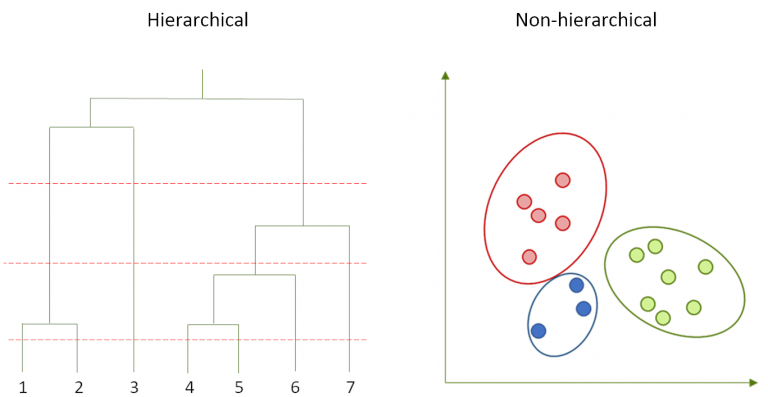
\includegraphics[scale=0.3]{victoria/compJerarquicoNoJerarquico}
		\caption{Comparación métodos jerárquico y no jerárquico.}
		\label{fig:ejemplo_metodos}
	\end{figure}

\end{frame}

\section{Métodos de agrupamiento\\ Jerárquicos}
\begin{frame}{Métodos Jerárquicos}
	\centering
	\textbf{Definición} método de análisis de grupos puntuales, que se basa en buscar una construcción de una jerarquía de grupos. Se minimizan las distancias y no es necesario conocer el número de grupos que se van a formar.\\
	\begin{figure}[H]
		\centering
		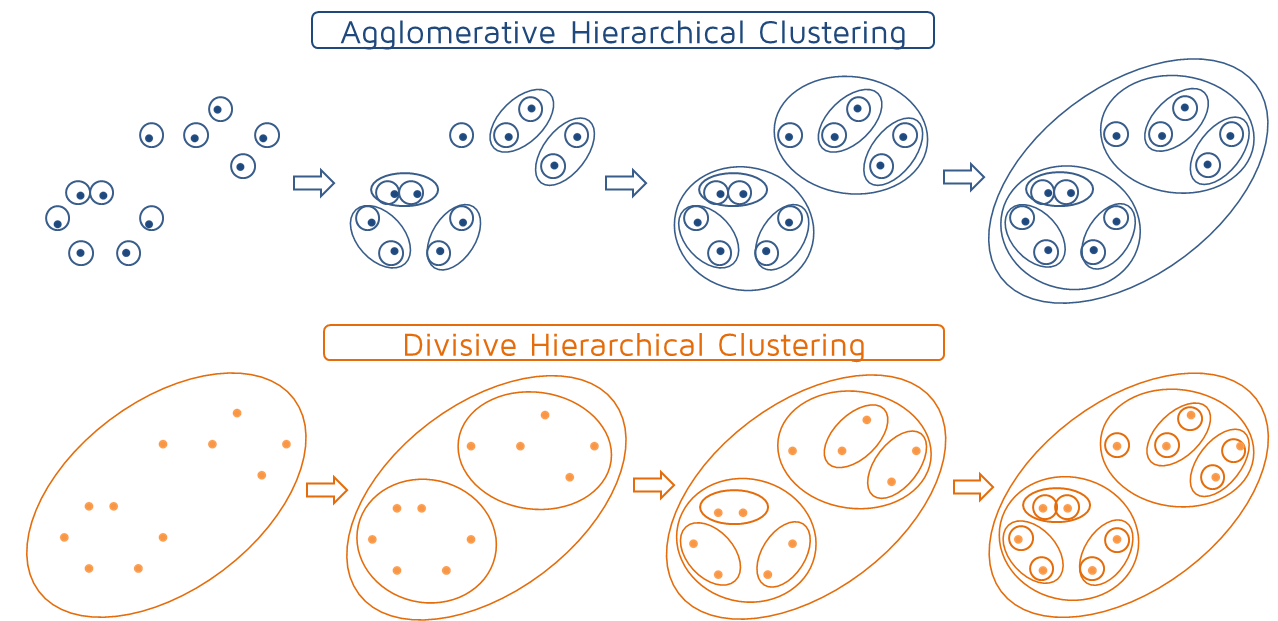
\includegraphics[scale=0.15]{victoria/compAglomeDivisivo}
		\caption{Comparación métodos aglomerativos y divisivos.}
		\label{fig:agl_div}
	\end{figure}
\end{frame}

\begin{frame}{Comparación de técnicas aglomerativas y divisivas}

	\begin{figure}[H]
	\centering
	\begin{subfigure}[b]{.4\textwidth}
		  \centering
	  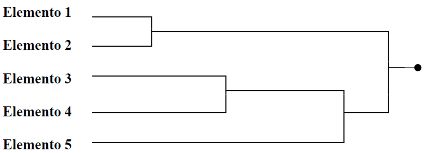
\includegraphics[width=\textwidth]{victoria/aglomerativo}
	  \caption{Ejemplo de dendrograma aglomerativo.}
	  \label{fig:aglomerativo}
	\end{subfigure}
	\begin{subfigure}[b]{.4\textwidth}
	  \centering
	  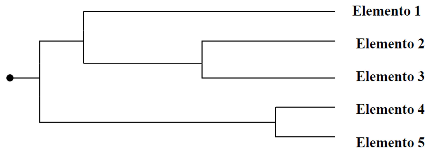
\includegraphics[width=\textwidth]{victoria/disociativo}
	  \caption{Ejemplo de dendrograma divisivo.}
	  \label{fig:divisivo}
	\end{subfigure}
	\caption{Comparación de dendrogramas aglomerativos y divisivo}
	\label{fig:compDendro}
	\end{figure}

\end{frame}

\begin{frame}{Ejemplo \textit{Single Link Method}}

	\textbf{Distancia entre dos clústers}

	\begin{equation}\label{eq:distAgloEjm}
		d(R, S) = min \{d_{rs}\ :\ r \in R, \ s \in S\}
	\end{equation}


\end{frame}

\begin{frame}{Ejemplo \textit{Single Link Method}}

	\textbf{Matriz de distancias}
	\[ \mathcal{D} =
	\left[ \begin{array}{c}
	d_{rs}
	\end{array} \right] =
	\begin{blockarray}{cccccc}
		& 1 & 2 & 3 & 4 & 5 \\
		\begin{block}{c[ccccc]}
			\\
			1 & 0 & 2 & 4 & 7 & 9 \\
			2 & 2 & 0 & 8 & 9 & 8 \\
			3 & 4 & 8 & 0 & 3 & 7 \\
			4 & 7 & 9 & 3 & 0 & 5 \\
			5 & 9 & 8 & 7 & 5 & 0 \\
			\\
		\end{block}
	\end{blockarray}  
	\] 

\end{frame}

\begin{frame}{Ejemplo \textit{Single Link Method}}

	\textbf{Matriz de distancias}
	\[ \mathcal{D} =
	\left[ \begin{array}{c}
	d_{rs}
	\end{array} \right] =
	\begin{blockarray}{cccccc}
		& 1 & 2 & 3 & 4 & 5 \\
		\begin{block}{c[ccccc]}
			\\
			1 & 0 & \textbf{2} & 4 & 7 & 9 \\
			2 & \textbf{2} & 0 & 8 & 9 & 8 \\
			3 & 4 & 8 & 0 & 3 & 7 \\
			4 & 7 & 9 & 3 & 0 & 5 \\
			5 & 9 & 8 & 7 & 5 & 0 \\
			\\
		\end{block}
	\end{blockarray}  
	\] 

 Tomamos los clúster \textit{1} y \textit{2} y formamos el nuevo clúster \textit{(12)}
\end{frame}

\begin{frame}{Ejemplo \textit{Single Link Method}}

	Cálculo de las nuevas distancias
	\begin{center}
	$d_{(12)(3)}$ = min\{$d_{13}$, $d_{23}$\} = min \{4, 8\} = 4\\
	$d_{(12)(4)}$ = min\{$d_{14}$, $d_{24}$\} = min \{7, 9\} = 7\\
	$d_{(12)(5)}$ = min\{$d_{15}$, $d_{25}$\} = min \{9, 8\} = 8\\
	\end{center}
\end{frame}

\begin{frame}{Ejemplo \textit{Single Link Method}}

	\textbf{Matriz de distancias}
	\[ \mathcal{D}_1  =
	\begin{blockarray}{ccccc}
		& (12) & 3 & 4 & 5 \\
		\begin{block}{c[cccc]}
			\\
			(12) & 0 & 4 & 7 & 8 \\
			3 & 4 & 0 & \textbf{3} & 7 \\
			4 & 7 & \textbf{3} & 0 & 5 \\
			5 & 8 & 7 & 5 & 0 \\
			\\
		\end{block}
	\end{blockarray}  
	\]
	Tomamos los clúster \textit{3} y \textit{4} y formamos el nuevo clúster \textit{(34)}
\end{frame}

\begin{frame}{Ejemplo \textit{Single Link Method}}

	Cálculo de las nuevas distancias\\
	\begin{center}
		$d_{(34)(12)}$ = min\{$d_{(3)(12)}$, $d_{(4)(12)}$\} = min \{4, 7\} = 4\\
		$d_{(34)(5)}$ = min\{$d_{(3)(5)}$, $d_{(4)(5)}$\} = min \{7, 5\} = 5\\
	\end{center}
\end{frame}

\begin{frame}{Ejemplo \textit{Single Link Method}}
	\textbf{Matriz de distancias}
	\[ \mathcal{D}_2  =
	\begin{blockarray}{cccc}
		& (12) & (34) & 5 \\
		\begin{block}{c[ccc]}
			\\
			(12) & 0 & \textbf{4} & 8 \\
			(34) & \textbf{4} & 0 & 5 \\
			5 & 8 & 5 & 0 \\
			\\
		\end{block}
	\end{blockarray}  
	\] 
	Tomamos los clúster \textit{(12)} y \textit{(34)} y formamos el nuevo clúster \textit{(1234)}
\end{frame}

\begin{frame}{Ejemplo \textit{Single Link Method}}

	Cálculo de la nueva distancia
	\begin{center}
	$d_{(12)(34)5}$ = min\{$d_{(12)(5)}$, $d_{(34)(5)}$\} = min \{8, 5\} = 5
	\end{center}
	Finalmente se obtiene el clúster \textit{(12345)}
\end{frame}

\begin{frame}{Ejemplo \textit{Single Link Method}}
	\begin{figure}[H]
		\centering
		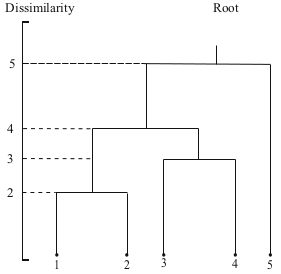
\includegraphics[scale=0.56]{victoria/agloEjem}
		\caption{Dendrograma ejemplo \textit{Single Link}.}
		\label{fig:agloEjem}
	\end{figure}
\end{frame}



\section{Métodos de agrupamiento\\ Particionamiento}



\section{Número de clústeres}
\begin{frame}{Número de clústeres}
	\begin{itemize}
		\item En los algoritmos de \textit{clustering}, uno de los problemas es determinar el número idóneo de clústeres $ k $. 
		\item Es un proceso ambiguo. Depende de las interpretaciones según la forma y la escala de de la distribución de los datos y la solución deseada.
		\item Como $ k $ decrece de $ n $ a 1, el valor de la distancia debería aumentar ya que tendría que ser mayor cuando dos clústeres distintos se agrupan en uno solo.
	\end{itemize}
\end{frame}

\begin{frame}{Número de clústeres-Método del codo}
	Consiste en dibujar la gráfica de las distancia a los centros de cada clúster en función del número de clústeres. Definimos:
	\[
	SSE_k = \sum_{i = 1}^{n_k} = \norm{\yy_i - \bar{\yy}_k}^2,
	\]
	y para cada $ k $ dibujamos
	\[
	D_k = \sum_{i = 1} ^ {k} SSE_k.
	\]
\end{frame}

\begin{frame}{Número de clústeres-Método del codo}
	\begin{figure}[h]
		\centering
		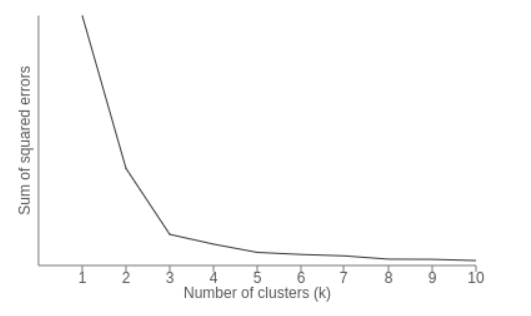
\includegraphics[scale=0.5]{pedro/elbowGraph}
		\caption{Ejemplo del método del codo.}
		\label{smkm}
	\end{figure}
\end{frame}

\begin{frame}{Número de clústeres-Estadístico $ R^2 $}
	Para $ n $ clústeres la suma total de las distancias al cuadrado es $ T = \sum_{i = 1}^{n} \norm{\yy_i - \bar{\yy}}^2 $. Así, para $ k $ clústeres definimos $ R^2 $ como
	\[
	R^{2}_{k} = \frac{T - \sum_k SSE_k}{T}.
	\]
	Para $ n $ clústeres $ SSE_k = 0 $ por lo que $ R^2 = 1 $. Una gran disminución en $ R^2_k $ representaría un agrupamiento diferente. \\
	También podríamos tener en cuenta el cambio en $ R^2 $ al unir los clústeres $ R $ y $ S $ como $ SR^2 = R_k^2 - R^2_{k-1} $. El estadístico $ SR^2 $ representa, en función de $ T $, la proporción de $ SSE_t - (SSE_r + SSE_s) $ donde los clústeres $ C_R $ y $ C_S $ se han unido para formar el clúster $ C_T $.  Cuanto mayor sea el índice mayor será la pérdida de homogeneidad.
\end{frame}

\begin{frame}{Número de clústeres-Varianza agrupada}
	Para un solo clúster \[ s^2 = \sum_{i=1}^{n} \norm{\yy_i - \bar{\yy}}^2/ p(n-1).\]
	Para el clúster $ C_k $
	\[
	s^2 = \sum_{i=1}^{n_k} \norm{\yy_i - \bar{\yy}_k}^2/ p(n_k-1).
	\]
	Valores grandes de la varianza agrupada indica que los clústeres no son homogéneos. Por lo tanto, si tiende a cero para algún $  k < n $ indica la formación de un clúster homogéneo.
\end{frame}

\begin{frame}{Número de clústeres-Pseudo estadísticos}
	El pseudo estadístico $ F $ se define como
	\[
	F^*_k = \frac{(T-\sum_k SSE_k) / (k-1)}{\sum_k SSE_k / (n-k)}.
	\]
	El pseudo estadístico $ t^2 $ se define como
	\[
	\text{pseudo }t^2 = \frac{\lbrack SSE_t - (SSE_r + SSE_s)\rbrack(n_R + n_S - 2)}{SSE_r + SSE_s}.
	\]
\end{frame}

\begin{frame}{Número de clústeres-\textit{Silhouette method}}
	Definimos el índice:
	\[
	s(i) = \frac{b(i)-a(i)}{\max\{b(i), a(i)\}}, \hspace{2mm} \forall i = 1, \dots, n
	\] 
	donde 
	\[
	a(i) = \frac{1}{|C_i|-1}\sum_{j\in C_i, j \neq i} d(i,j) 
	\]	y
	\[
	b(i) = \min_{k \neq i} \frac{1}{|C_k|} \sum_{j \in C_k} d(i,j).
	\] 
	Se escoge el $ k $ que maximice el valor medio de $ s(i) $.
\end{frame}

\begin{frame}{Número de clústeres-\textit{Silhouette method}}
	\begin{table}[h!]
		\centering
		\begin{tabular}{cc} 
			\hline
			k & Silhouette coeff. \\
			\hline
			2 &  0.7049787496083262 \\			 
			3 & 0.5882004012129721 \\	
			4 &  0.6505186632729437 \\
			5 &  0.5745566973301872 \\
			6 & 0.43902711183132426 \\
			\hline
		\end{tabular}
		\caption{Ejemplo \textit{silhouette method}.}
	\end{table}
	Vemos que se obtienen los mejores resultados con 2 o 4 clústeres.
\end{frame}

\begin{frame}{Número de clústeres-\textit{Gap method}}
	El $ k $ elegido será aquel que maximice el valor de:
	\[
	Gap(k) = E^*_n\{ \log(W_k)\} - \log(W_k).
	\]
	En la fórmula anterior $ E^*_n $ denota la media de una de muestra de tamaño $ n $ y 
	\[
	W_k = \sum_{R = 1}^{k}\frac{1}{2 n_R}\sum_{i j \in C_R} d(i,j).
	\]
\end{frame}

\begin{frame}{Número de clústeres-\textit{Gap method}}
	\begin{figure}[H]
		\centering
		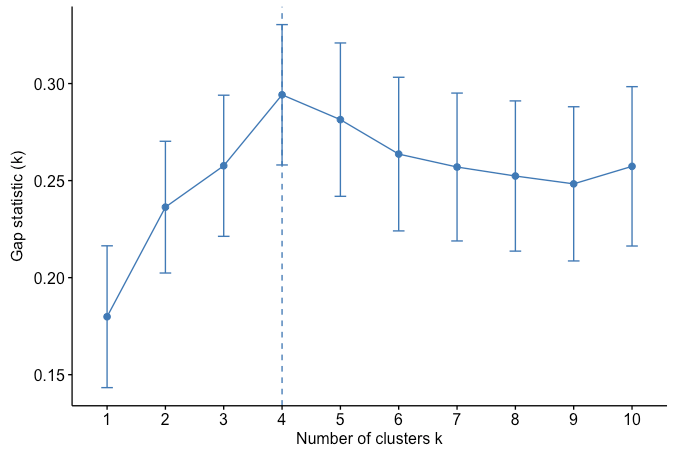
\includegraphics[scale=0.32]{pedro/gapGraph}
		\caption{Ejemplo del método de la brecha.}
	\end{figure}
\end{frame}

%%% Parte Práctica

\begin{frame}{\textit{Caso de estudio : Flor de Iris}}

Estudiaremos el conjunto de datos iris de \textbf{Fisher}.\break

Contiene 50 muestras de cada una de tres especies de flor \textbf{Iris}. Para cada muestra, se recogen las medidas de: largo y ancho del sépalo y y largo y ancho del pétalo, en centímetros.

\begin{figure}[h]
  \centering
  \begin{minipage}[h]{0.28\textwidth}
    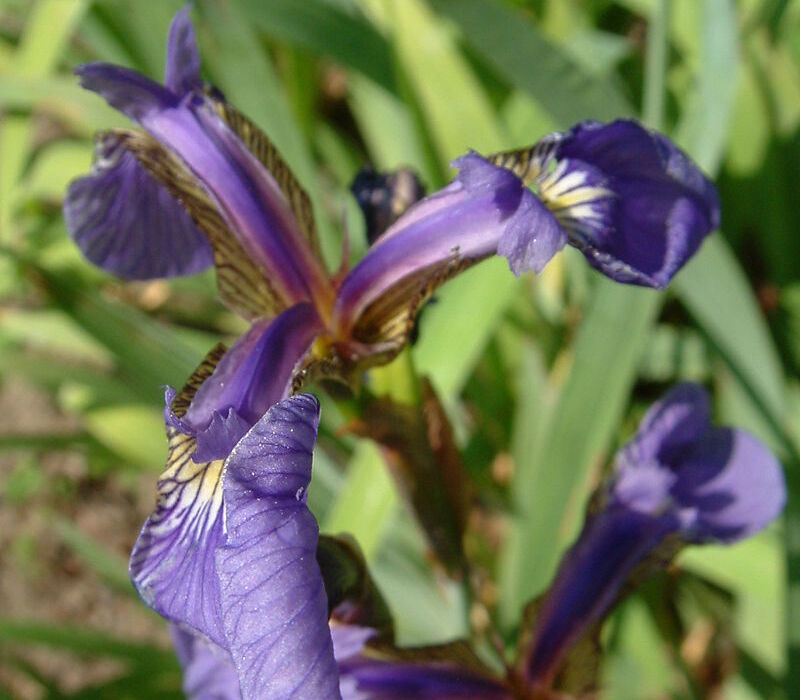
\includegraphics[width=\textwidth]{dani/setosa.jpg}
    \caption{Iris Setosa.}
  \end{minipage}
  \hfill
  \begin{minipage}[h]{0.28\textwidth}
    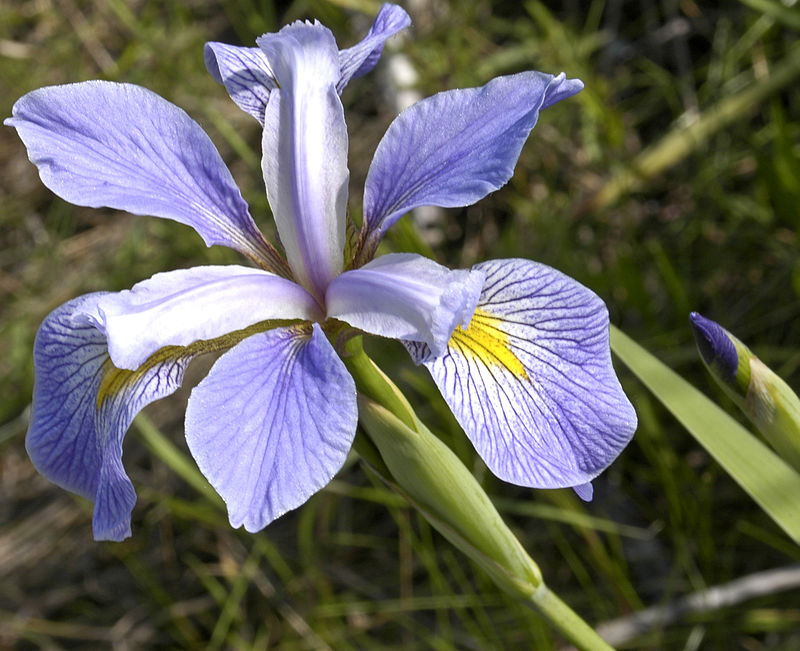
\includegraphics[width=\textwidth]{dani/virginica.jpg}
    \caption{Iris virginica.}
  \end{minipage}
  \hfill
  \begin{minipage}[h]{0.29\textwidth}
    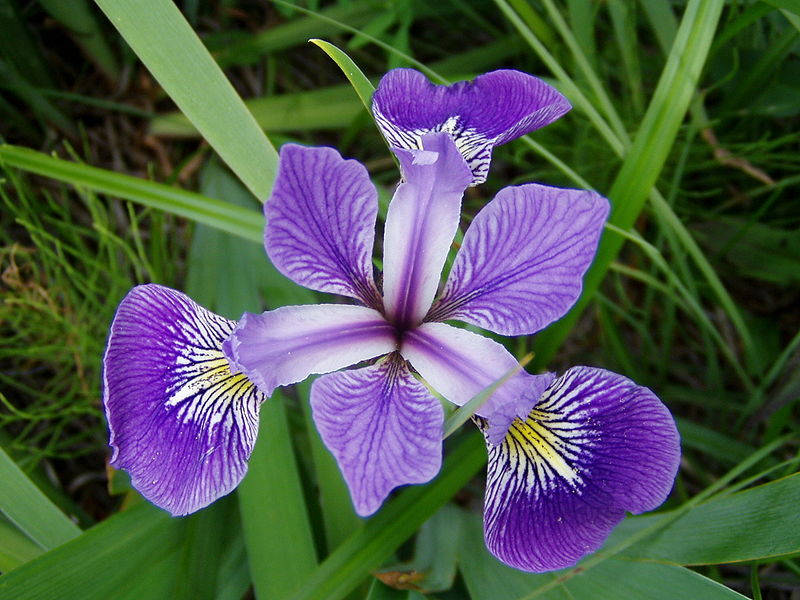
\includegraphics[width=\textwidth]{dani/versicolor.jpg}
    \caption{Iris versicolor.}
  \end{minipage}
\end{figure}
\end{frame}

\begin{frame}{\textit{Métricas utilizadas}}

Se utilizarán las siguientes métricas para medir la bondad de los algoritmos:\break
\begin{itemize}
\item \textbf{Calinski-Harabaz}: Nos indica si estamos usando un buen número de clústeres para un algoritmo en concreto. El número óptimo de clústeres tendrá la solución con el valor de Calinski-Harabasz más alto.
\item \textbf{Silhouette}: Cuanto mayor sea su valor, más similar será un objeto respecto a su grupo y más diferente a los de otros clúster. Toma valores entre -1 y +1. Si el valor es cercano a 1, la configuración de los clúster es apropiada, si no, habrá más o menos clústeres de los necesarios.
\end{itemize}
\end{frame}

\begin{frame}{\textit{Tabla comparativa de los algoritmos}}

Las mejores configuraciones son las que hayan obtenido un mayor valor del coeficiente de Silhouette.

\begin{table}[H]
\centering
\resizebox{9cm}{!} {
\begin{tabular}{lrrrrr}
\toprule
\textbf{Nombre} & \textbf{Nº clústeres} & \textbf{CH} & \textbf{SH} & \textbf{Tiempo ($s$)} & \textbf{Clústeres}                                                                                                          \\ \midrule
K-Means       & 3                    & 359.845074 & 0.504769    & 0.016456      & \begin{tabular}[c]{@{}c@{}}0:    61 (40.67\%)\\
1:    50 (33.33\%) \\2:    39 (26.00\%)\end{tabular}\\ \\
DBSCAN        & 4                   &  94.991819   & 0.306404   &  0.002353      & \begin{tabular}[c]{@{}c@{}}0:    45 (30.00\%)
\\1:    39 (26.00\%)
\\-1:    36 (24.00\%)
\\2:    30 (20.00\%)\end{tabular} \\ \\
AggCluster    & 3                    & 349.254185 & 0.504800    & 0.019058      & \begin{tabular}[c]{@{}c@{}}0:    67 (44.67\%)
\\1:    50 (33.33\%)
\\2:    33 (22.00\%)\end{tabular}                       \\ \\
MeanShift     & 3                    & 290.470683  & 0.476961    & 0.289073      & \begin{tabular}[c]{@{}c@{}}0:    81 (54.00\%)
\\1:    50 (33.33\%)
\\2:    19 (12.67\%)\end{tabular}                                             \\ \bottomrule
\end{tabular}
}
\end{table}
\end{frame}

\begin{frame}{Gráficas}
Para cada algoritmo, se mostrarán algunas gráficas que nos ayudarán a comprender como funciona el agrupamiento para el caso de estudio.\break

Las gráficas utilizadas serán \textbf{Scatter Matrix, Heatmap, KPlot y BoxPlot} que mostrarán la matriz de dispersión de las muestras, mapa de calor de los centroides para cada variable y distribución de las muestras según cada variable.\break

Para el caso del algoritmo \textbf{Agglomerative Clustering} mostraremos como se forman los distintos clústers a partir del Dendrograma generado.
\end{frame}

\begin{frame}[fragile]
\frametitle{K-Means}
Para el algoritmo K-Means se ha utilizado el siguiente código en python y se ha obtenido la siguiente agrupación de las muestras:\break
\begin{lstlisting}
KMeans(init='k-means++', n_clusters=3, 
	n_init=5, random_state=12345)

cluster 0: 61 (40.67%)
cluster 1: 50 (33.33%)
cluster 2: 39 (26.00%)
\end{lstlisting}
\end{frame}

\begin{frame}
\begin{figure}[h]
\centering
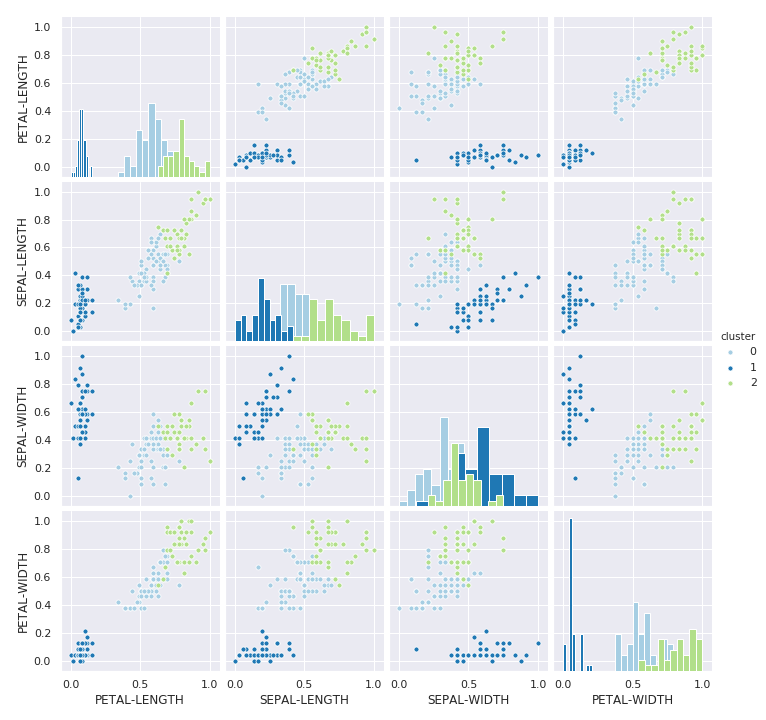
\includegraphics[scale=0.34]{dani/scatmatrixK-MeansIRIS.png}
\end{figure}
\end{frame}

\begin{frame}
\begin{figure}[h]
\centering
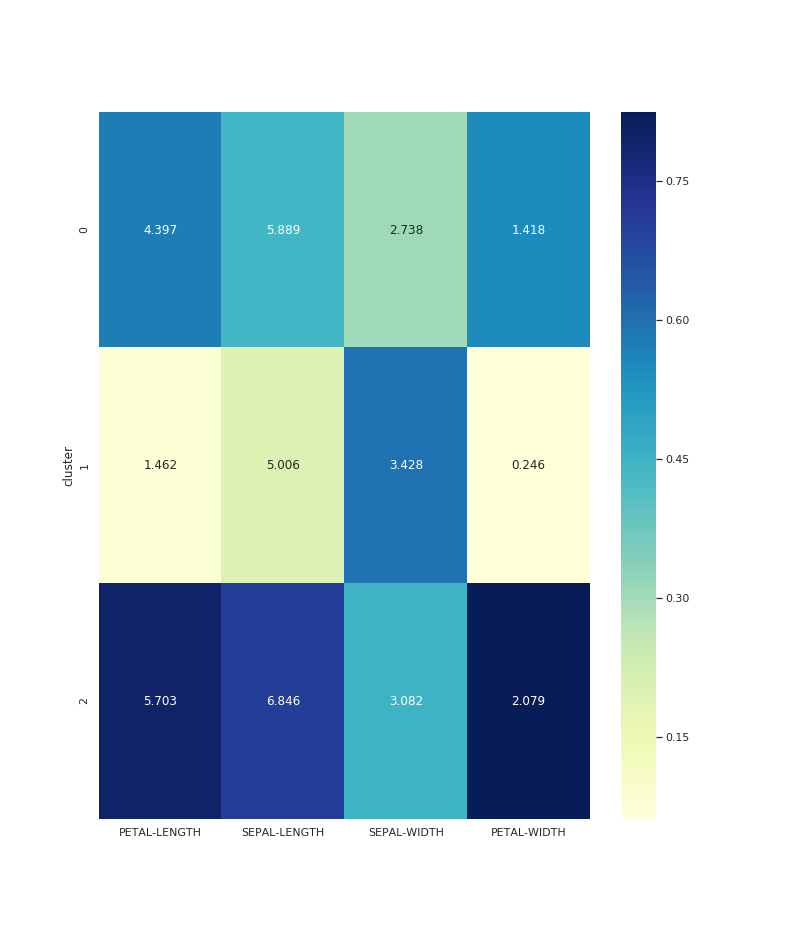
\includegraphics[scale=0.29]{dani/heatmapK-MeansIRIS.png}
\end{figure}
\end{frame}

\begin{frame}
\begin{figure}[h]
\centering
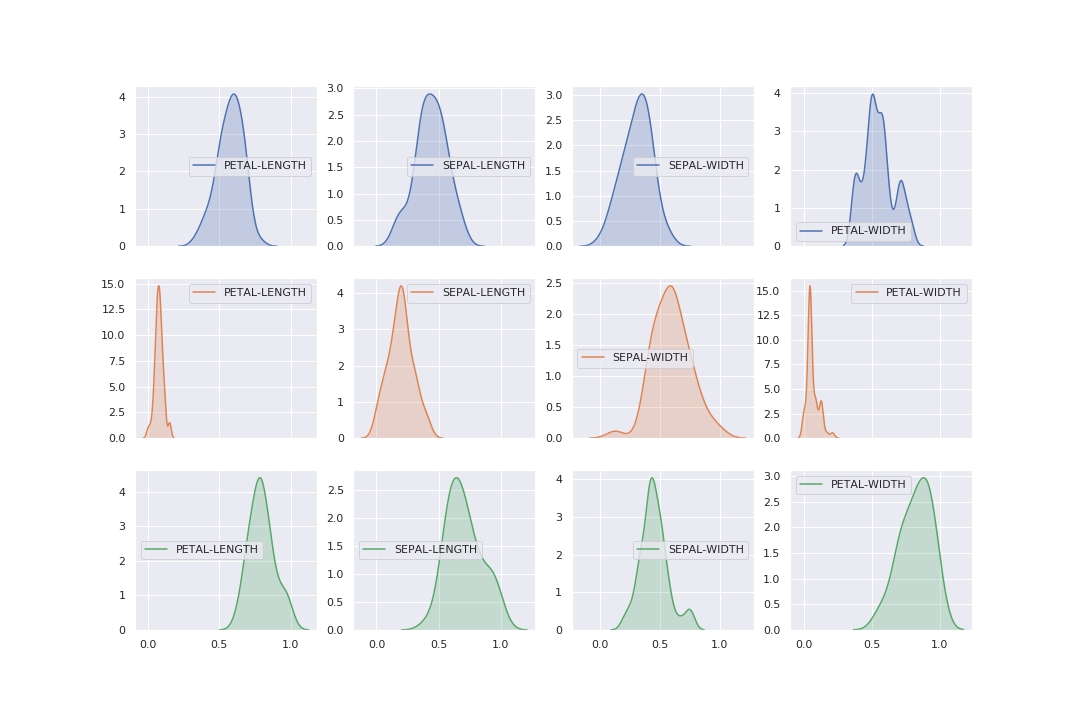
\includegraphics[scale=0.29]{dani/kdeplotK-MeansIRIS.png}
\end{figure}
\end{frame}

\begin{frame}
\begin{figure}[h]
\centering
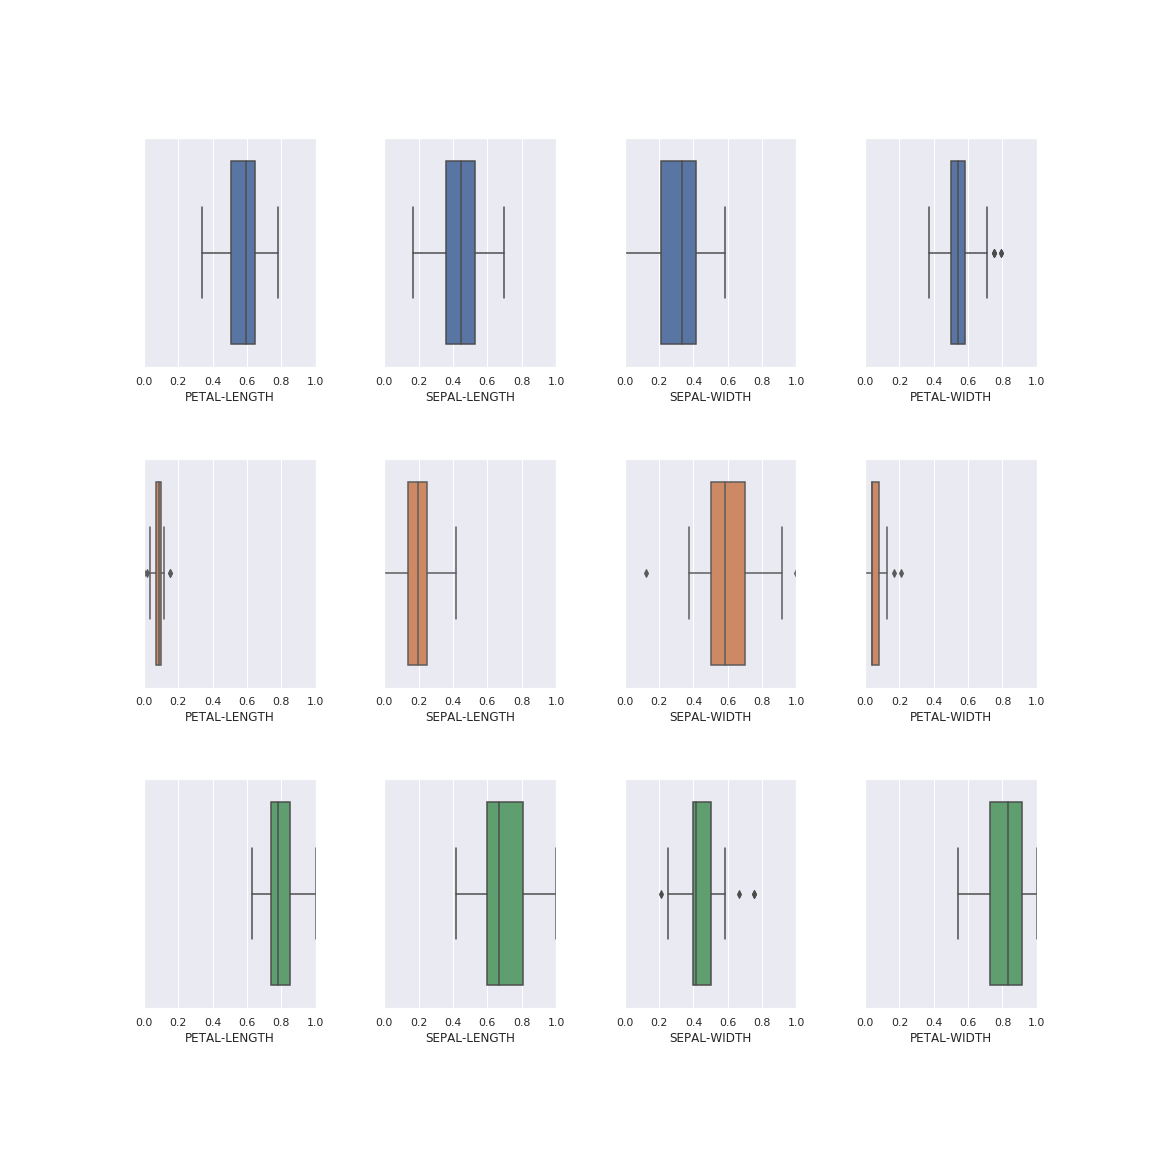
\includegraphics[scale=0.24]{dani/boxplotK-MeansIRIS.png}
\end{figure}
\end{frame}

\begin{frame}[fragile]
\frametitle{Agrupamiento Jerárquico}
Para el algoritmo Aglomerativo Jerárquico, se ha utilizado el siguiente código en python y se ha obtenido la siguiente agrupación de las muestras:\break
\begin{lstlisting}
AgglomerativeClustering(n_clusters=3, 
	linkage="ward", affinity='euclidean')

cluster 0: 67 (44.67%)
cluster 1: 50 (33.33%)
cluster 2: 33 (22.00%)
\end{lstlisting}
\end{frame}

\begin{frame}
\begin{figure}[h]
\centering
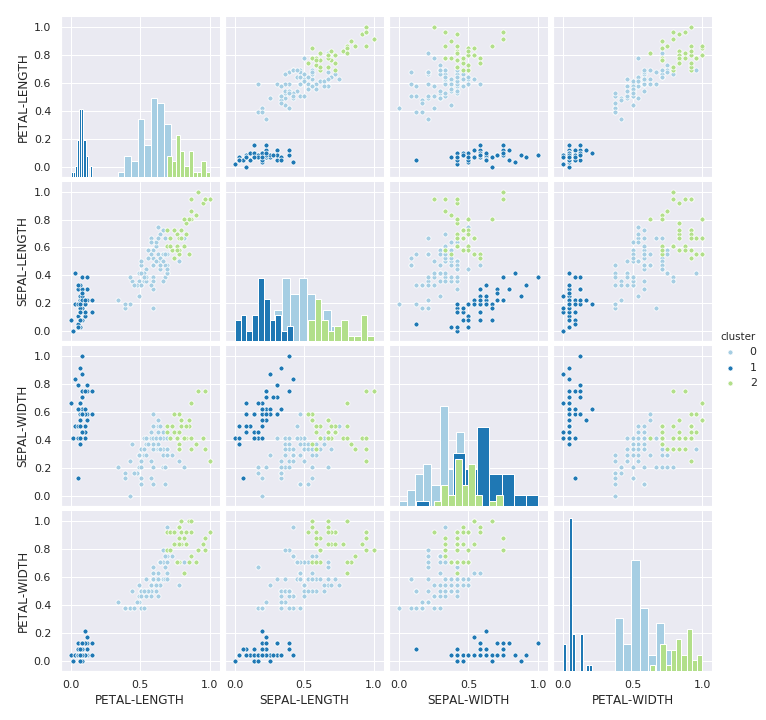
\includegraphics[scale=0.34]{dani/scatmatrixAggClusterIRIS.png}
\end{figure}
\end{frame}

\begin{frame}
\begin{figure}[h]
\centering
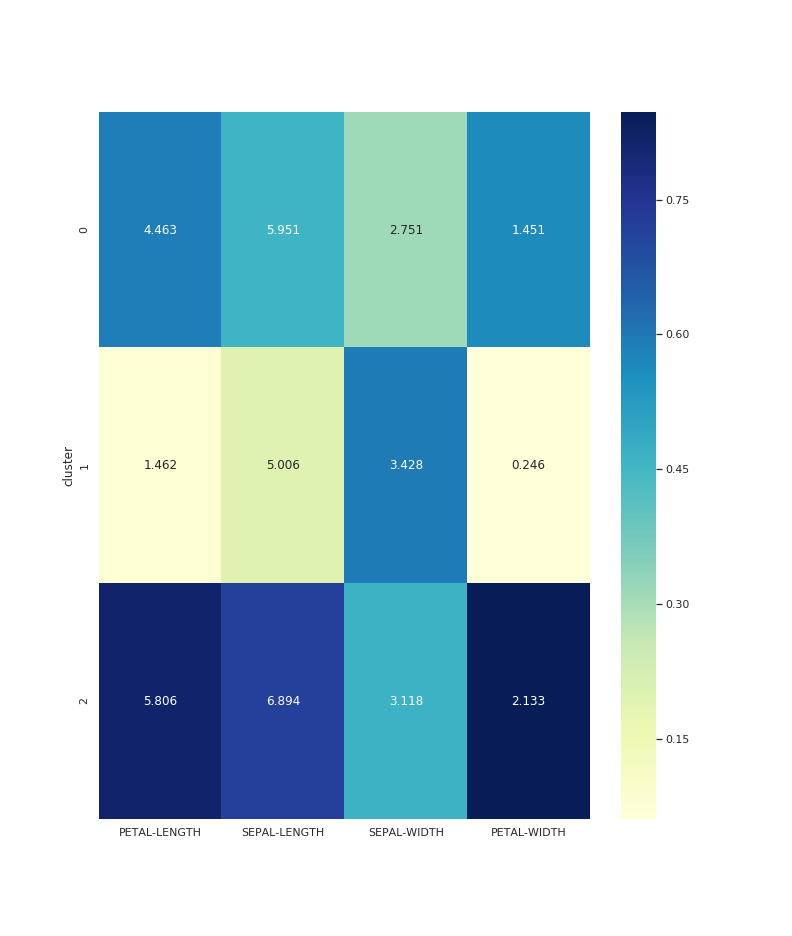
\includegraphics[scale=0.29]{dani/heatmapAggClusterIRIS.png}
\end{figure}
\end{frame}

\begin{frame}{\textit{Dendrogramas}}
Un \textbf{dendrograma} es un diagrama de árbol que muestra los grupos que se forman al crear clústers de observaciones en cada paso y sus niveles de similitud.\break

La decisión acerca de la agrupación final también se conoce como cortar el dendrograma. Cortar el dendrograma es similar a trazar una línea a lo largo del dendrograma para especificar la agrupación final.
\end{frame}

\begin{frame}
\begin{figure}[h]
\centering
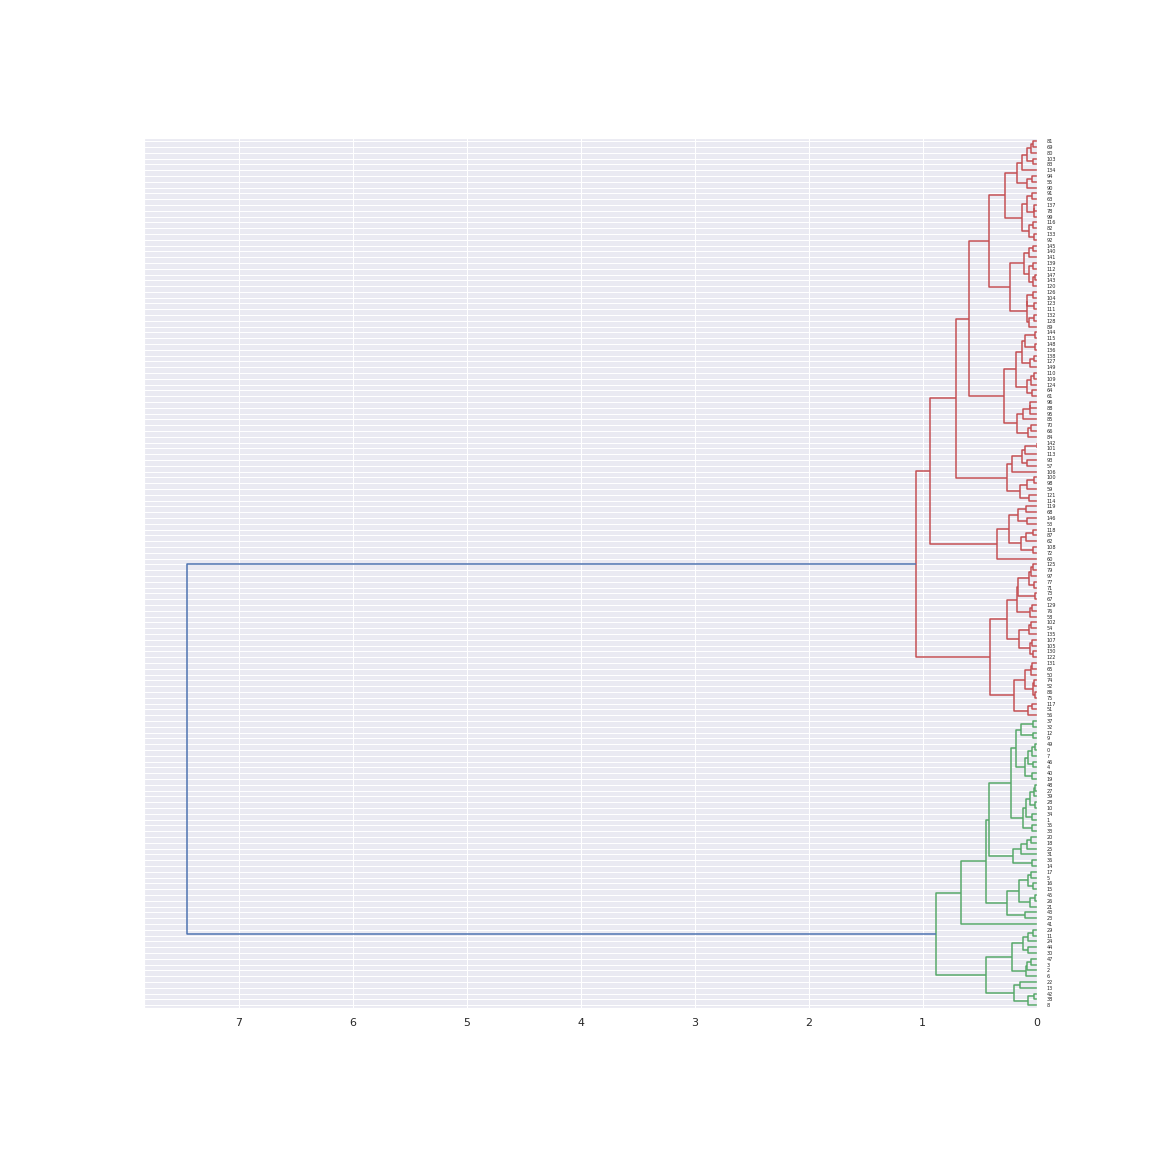
\includegraphics[scale=0.24]{dani/dendrogramAggClusterIRIS.png}
\end{figure}
\end{frame}

\begin{frame}
\begin{figure}[h]
\centering
\textbf{0}: 67 (44.67\%), \textbf{1}: 50 (33.33\%), \textbf{2}: 33 (22.00\%)
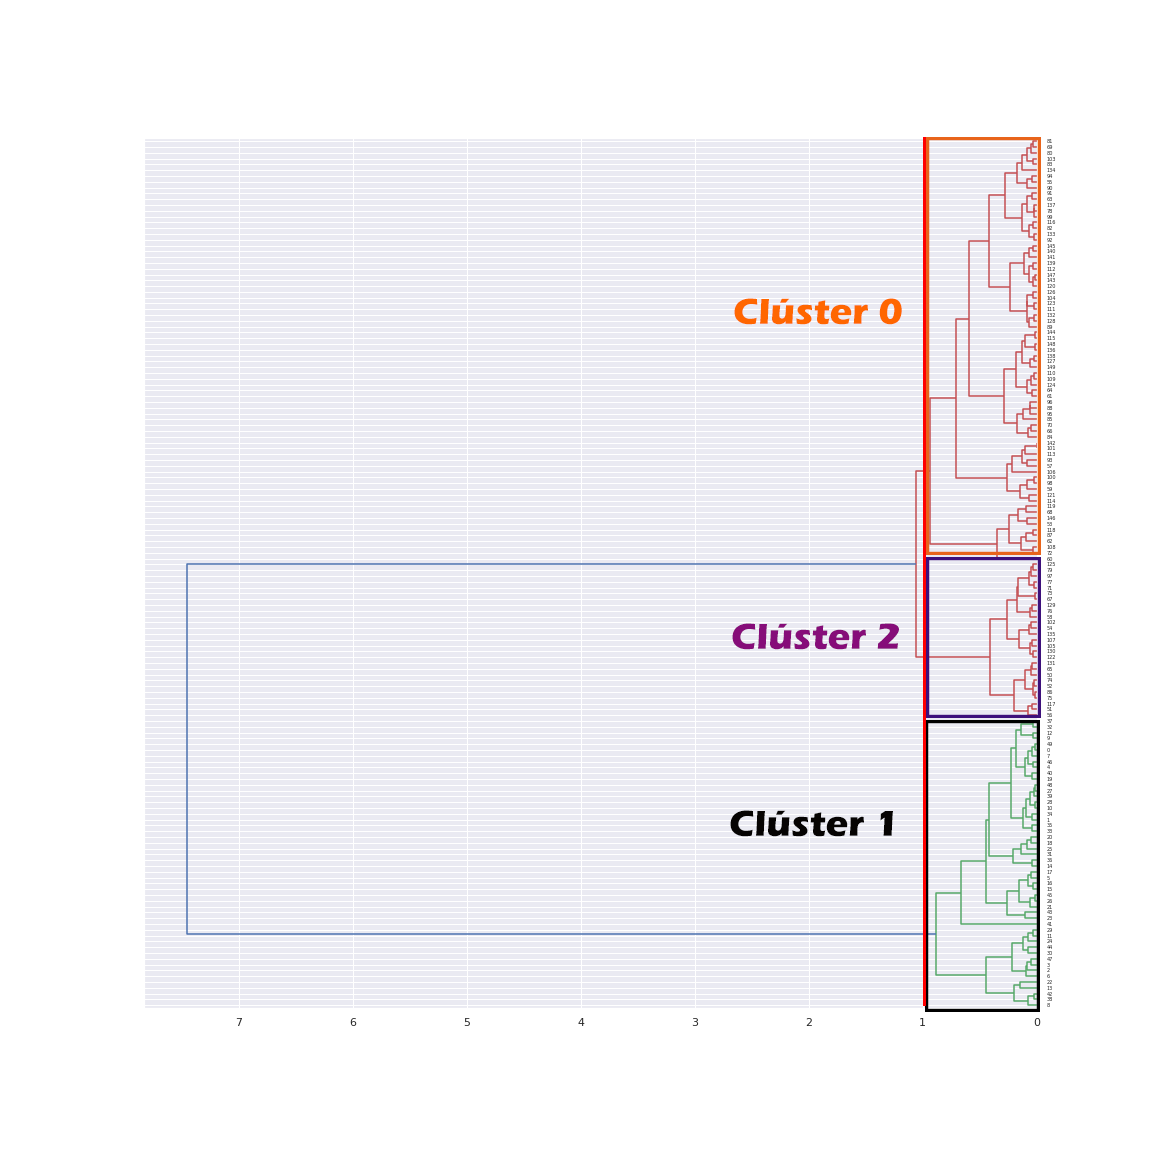
\includegraphics[scale=0.23]{dani/dendrogramcolor.png}
\end{figure}
\end{frame}

\begin{frame}{DBSCAN}
\begin{itemize}
\item Se basa en la densidad de las muestras para identificar los clústeres.
\item Los clústers pueden tener cualquier forma.
\item Dos parámetros para definir este algoritmo son: \textbf{eps} y \textbf{min\_samples}.
\end{itemize}
\begin{figure}[h]
\centering
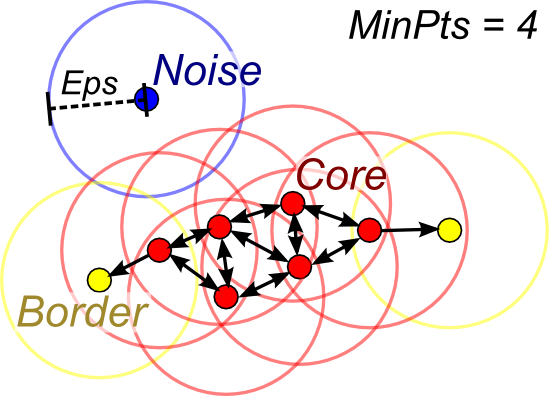
\includegraphics[scale=1.2]{dani/DBSCAN.png}
\end{figure}
\end{frame}

\begin{frame}{DBSCAN}
La técnica de agrupación DBSCAN clasifica los puntos como puntos núcleo, puntos (densamente-)alcanzables, o ruido de la siguiente forma:

\begin{itemize}
\item Un punto $p$ pertenece al núcleo si al menos \textit{min\_samples} puntos están a una distancia $\epsilon$ de él y esos puntos son directamente alcanzables desde $p$.
\item Un punto $q$ es alcanzable desde $p$ si existe una secuencia de puntos $p_1\dots p_n$ donde $p_1=p$ y $p_n=q$ y cada punto $p_{i+1}$ es directamente alcanzable desde $p_i$.
\item Un punto que no sea alcanzable desde cualquier otro se considera ruido.
\end{itemize}
\end{frame}

\begin{frame}{DBSCAN}
Un clúster generado por DBSCAN satisface dos propiedades:

\begin{itemize}
\item Todos los puntos de un mismo clúster están densamente conectados entre sí.
\item Si un punto $A$ es alcanzable desde cualquier otro punto $B$ del clúster, entonces $A$ también forma parte del clúster.
\end{itemize}
\begin{figure}[h]
\centering
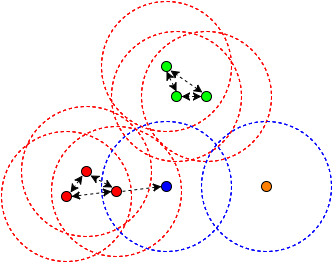
\includegraphics[scale=0.37]{dani/DBSCAN2.png}
\end{figure}
\end{frame}

\begin{frame}[fragile]
\frametitle{DBSCAN}
Para DBSCAN, se ha utilizado el siguiente código en python y se ha obtenido la siguiente agrupación de las muestras, donde el clúster -1 representa las muestras formadas por ruido:\break
\begin{lstlisting}
DBSCAN(eps=0.12, min_samples=5)

cluster 0:  45 (30.00%)
cluster 1:  39 (26.00%)
ruido  -1:  36 (24.00%)
cluster 2:  30 (20.00%)
\end{lstlisting}
\end{frame}

\begin{frame}
\begin{figure}[h]
\centering
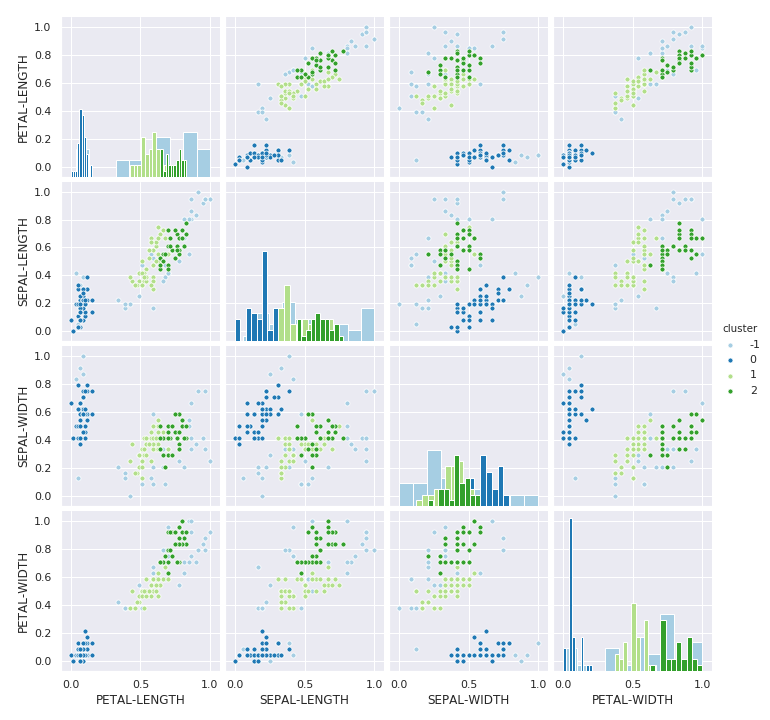
\includegraphics[scale=0.34]{dani/scatmatrixDBSCANIRIS.png}
\end{figure}
\end{frame}

\begin{frame}
\begin{figure}[h]
\centering
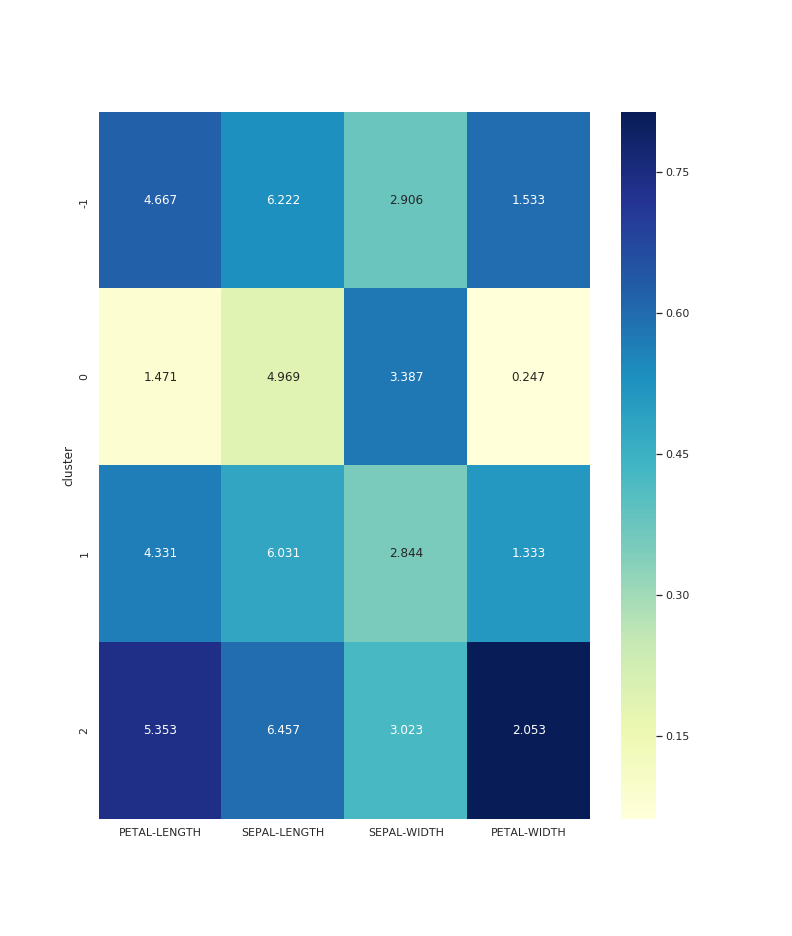
\includegraphics[scale=0.29]{dani/heatmapDBSCANIRIS.png}
\end{figure}
\end{frame}

\begin{frame}{Mean Shift}
Es una técnica de análisis de espacio de características no paramétrica para localizar los máximos de una función de densidad. 
\begin{itemize}
\item Método iterativo que parte de una estimación inicial $x$.
\item Define una función núcleo $K(x_i-x)$ que determina los pesos de los puntos cercanos para la reestimación media.
\end{itemize}\

La media ponderada de la densidad en $K$ es:

$$m(x)=\dfrac{\sum_{x_i\in N(x)}K(x_i-x)x_i}{\sum_{x_i\in N(x)}K(x_i-x)}$$

donde $N(x)$ es el vecindario de x, un conjunto de puntos donde $K(x_i)\neq0$.\\
\end{frame}

\begin{frame}{Mean Shift}
La diferencia $m(x)-x$ se denomina Mean Shift.\break

El algoritmo establece $m(x)\rightarrow x$ y repite la estimación hasta que $m(x)$ converja.\break

No existe ninguna prueba de la convergencia del algoritmo en espacios de alta dimensión y el caso unidimensional tiene aplicaciones limitadas en el mundo real.

\begin{figure}[h]
\centering
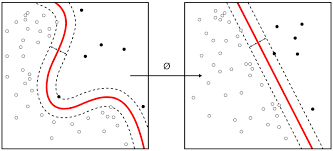
\includegraphics[scale=0.45]{dani/MS.png}
\end{figure}
\end{frame}

\begin{frame}{Mean Shift}
Sea un conjunto de datos finito $S$ embebido en el espacio euclídeo n-dimensional $X$. Sea $K$ un núcleo plano con función característica:

$$K(x)=\left\{
1 \ si \ ||x||\leq \lambda \atop
0 \ si \ ||x||> \lambda
\right.$$

En cada iteración del algoritmo, se establece $m(x)\rightarrow x$ para todo $s\in S$ a la vez.\break 

En un conjunto pequeño, estimaremos la función de densidad como:

$$f(x)=\sum_i K(x-x_i)=\sum_i k\dfrac{||x-x_i||^2}{h^2}$$

donde $x_i$ son las muestras de entrada y $k$ la función núcleo y h es el \textit{bandwidth}. 
\end{frame}

\begin{frame}{Mean Shift}
Una vez calculado $f(x)$ buscamos sus máximos locales utilizando el ascenso de gradiente o alguna otra técnica de optimización.\break

En problemas con grandes dimensiones, se usa la técnica del reinicio de gradiente descendiente múltiple, la cual empieza desde un máximo local $y_k$ y calcula su aproximación $f(x)$ avanzando en esa dirección.
\end{frame}

\begin{frame}[fragile]
\frametitle{Mean Shift}
Para Mean Shift, se ha utilizado el siguiente código en python y se ha obtenido la siguiente agrupación de las muestras:\break
\begin{lstlisting}
MeanShift(bandwidth=estimate_bandwidth(X_normal, 
	quantile=0.67, n_samples=400))

cluster 0: 81 (54.00%)
cluster 1: 50 (33.33%)
cluster 2: 19 (12.67%)
\end{lstlisting}
\end{frame}

\begin{frame}
\begin{figure}[h]
\centering
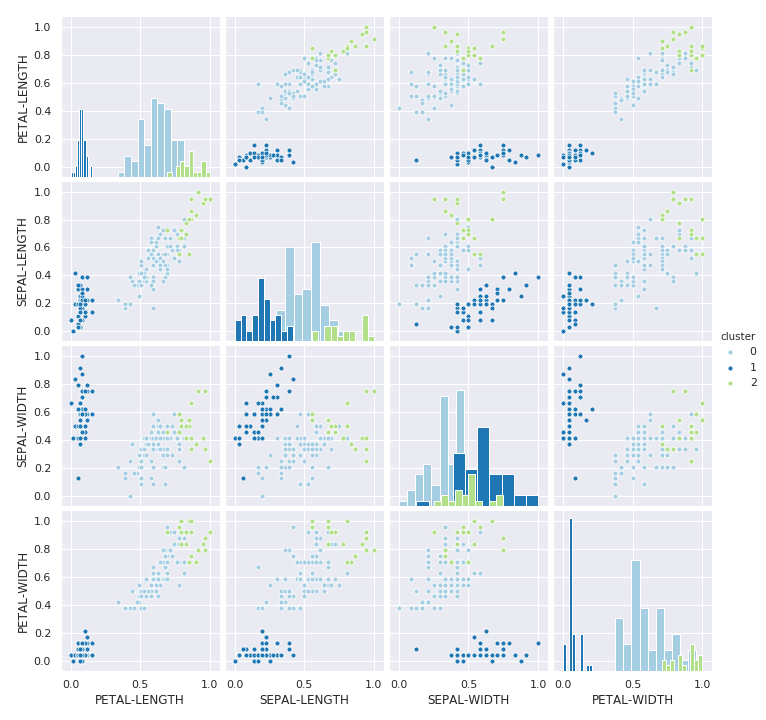
\includegraphics[scale=0.34]{dani/scatmatrixMeanShiftIRIS.png}
\end{figure}
\end{frame}

\begin{frame}
\begin{figure}[h]
\centering
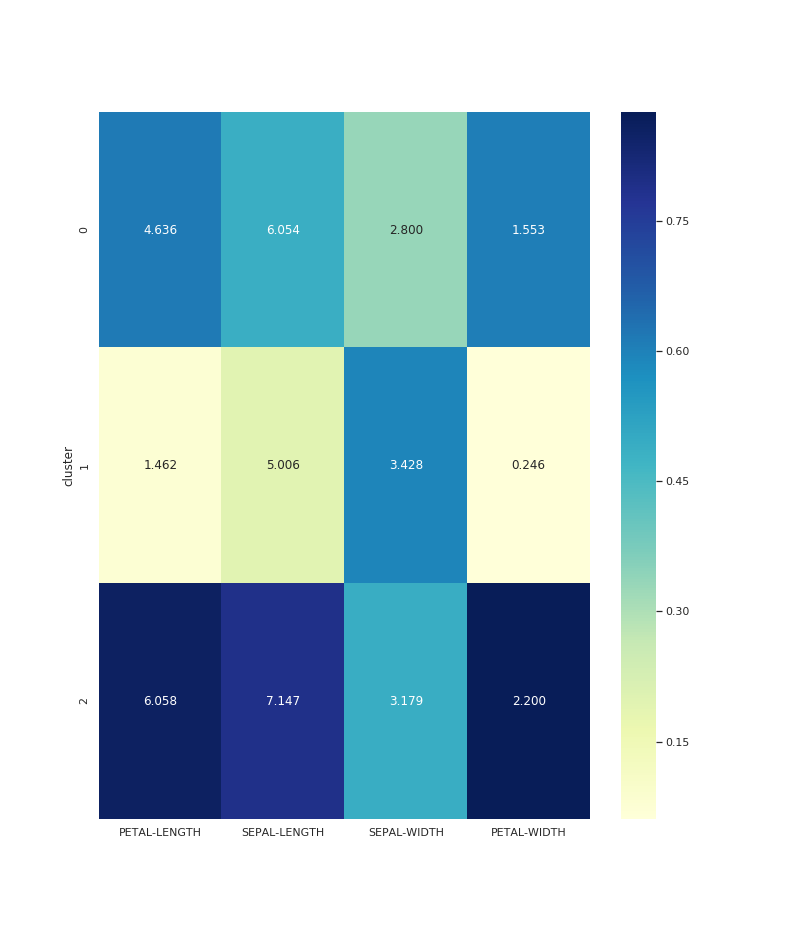
\includegraphics[scale=0.29]{dani/heatmapMeanShiftIRIS.png}
\end{figure}
\end{frame}

\begin{frame}[fragile, allowframebreaks]
  \frametitle{Referencias}
%  \nocite{*}
        \bibliographystyle{amsalpha}
        \bibliography{referencias_pres.bib}
\end{frame}
\end{document}

